\subsection{Vorteile von Angular [M]}
\setauthor{Fabian Maar}
Folgende Aspekte sprechen für die Nutzung von Angular in diesem Projekt:

\begin{itemize}
  \item komponentenbasiertes Programmieren um komplexe Benutzeroberflächen übersichtlich zu unterteilen;
  im Abschnitt Components \ref{components} wird nochmals deutlich, wie dieser Aspekt genutzt wird.
  \item einfache und übersichtliche Einbindung von Libraries durch ngModules; wird behandelt in Kapitel NgModules \ref{sec:NgModules} 
  \item Isolierung der Logik mit der Benutzeroberfläche durch die Model-View-Controller Architektur und die Model-View-ViewModel Architektur; wird behandelt in Kapitel MVC und MVVM \ref{sec:MVCandMVVM} 
  \item 
  Dependency Injection für die Verbindung von Front-End zum Back-End; siehe Kapitel HTTP Services \ref{DPI}
\end{itemize}

\subsubsection{Angular [M]}
\setauthor{Fabian Maar}
\begin{wrapfigure}{r}{0.3\textwidth}
  \begin{center}
    
\includegraphics[width=0.2\textwidth]{pics/AngularLogo.png}
   \caption{Angular Logo}
  \end{center}
\end{wrapfigure}
Angular ist ein Framework für Webapplikation, das auf der Programmiersprache Typescript basiert. Es ist eines der renommiertesten Frameworks zur Front-End-Entwicklung, wird als Open-Source-Software zur Verfügung gestellt und besitzt somit eine große Community. So zählt es 2022 zu dem zweitbeliebtesten Front-End Framework \cite{AngularEvidence} und wird von Milliardenkonzernen wie zum Beispiel Google oder PayPal verwendet. 
\cite{AngularEvidence2}

Die große Stärke von Angular ist die Erstellung von Single-Page-Webanwendung, da es eine komponentenbasierte Struktur besitzt. Das bedeutet, der Code ist wiederverwendbar und verkapselt. Komplexe Logiken werden auf ihre Grundelemente reduziert und beeinflussen sich nicht gegenseitig. \cite{AngularGeneral}

Angular basiert auf dem Konzept des Model-View-Controller- (MVC) und Model-View-ViewModel (MVVM) Architecture Patterns. Diese Patterns werden verwendet, um die Logik von der Benutzeroberfläche zu trennen und komplexe Aufgaben einfacher zu bewältigen. Dies wird in der Fachsprache auch oft als \emph{Seperation of Concerns} bezeichnet.
\cite{AngularArchitecturePattern} 

Architecture Patterns sind Muster, die verwendet werden,
\begin{itemize}
  \item eine Software-Anwendung zu strukturieren.
  \item die Redundanz von wiederholenden Code-Teile zu vermeiden.
  \item immer wiederkehrende Probleme durch eine einmalige Lösungen zu beheben.
  \item um die Wartung und Testung zu erleichtern.
  \item Änderungen am Umfang und der Größe der Applikation leichter handhaben zu können.
\end{itemize} \cite{MVCmdn, MVVM, MVC}

\paragraph{Model-View-Controler (MVC)}
Die \emph{Seperation of Concerns} wird bei diesem Pattern durch die Aufteilung der Applikation in Model, View und Controller realisiert. Dadurch ist es möglich, sich auf einen Aspekt der Implementierung zu fokussieren. 

\begin{figure} [h t]
  \centering
  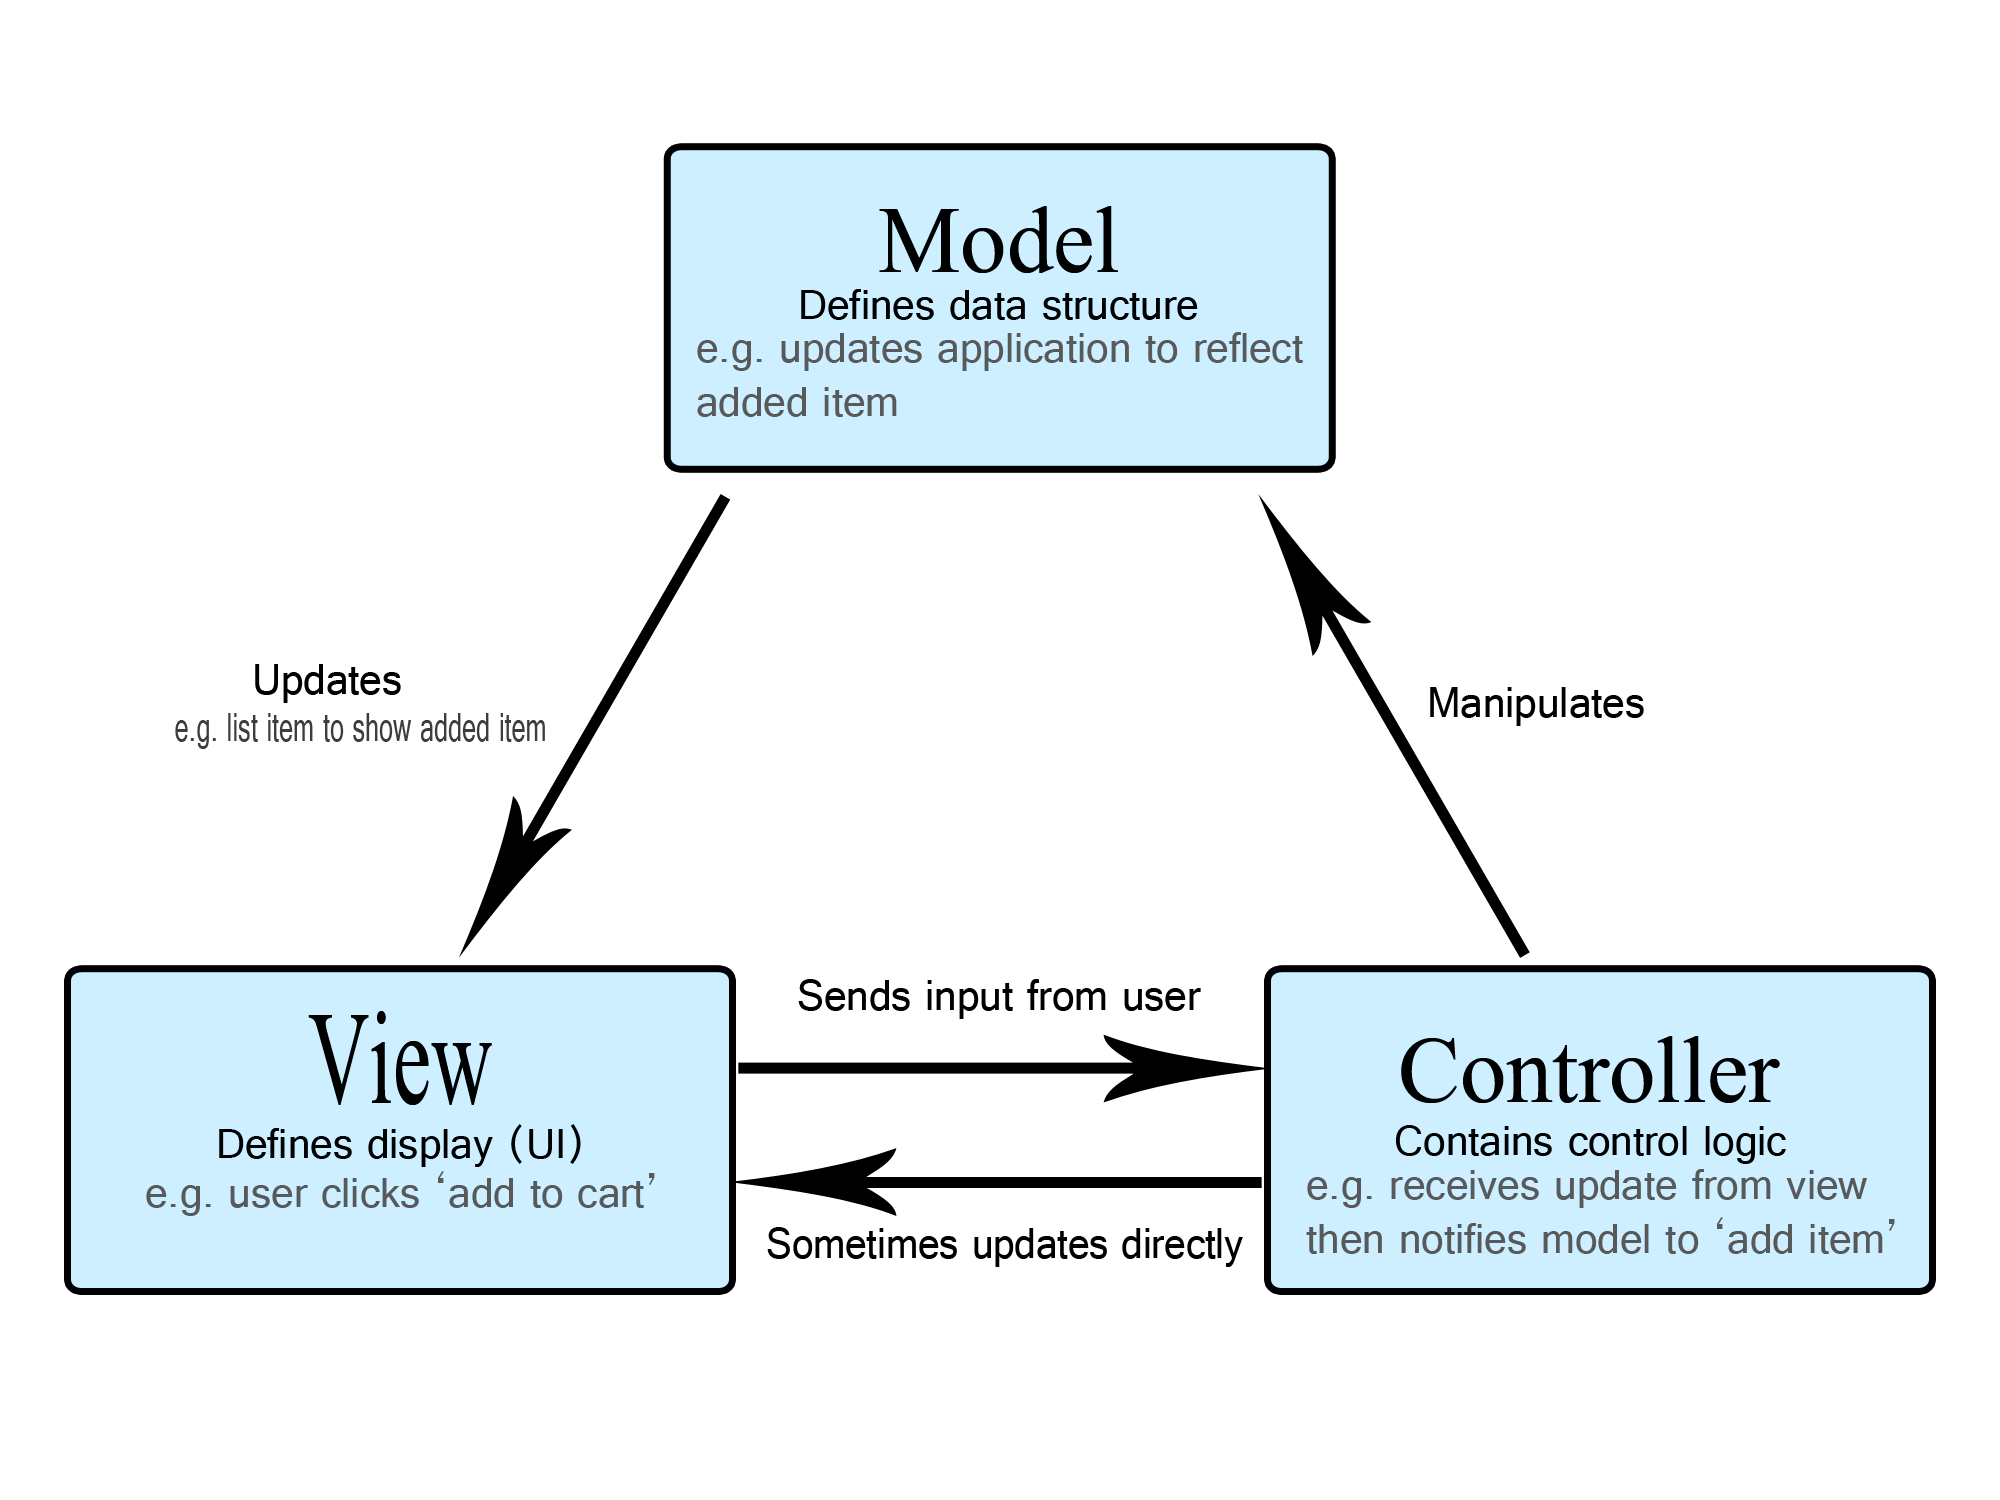
\includegraphics[scale=0.5]{pics/mvc.png}
  \caption{Die Model-View-Controller Pattern \cite{MVCmdn}}
  \label{fig:tech:front:mvc-architecture}
\end{figure}

Welche Daten eine Applikation beinhalten soll, wird über das Model geregelt. Falls sich das Model ändert, werden die Benutzerfläche und manchmal auch der Controller entsprechend geändert. In Angular sind diese Modelle mit den Interfaces (siehe Interfaces \ref{interface})  zu vergleichen.

\emph{View} ist die Benutzeroberfläche des Programms. Der*die Benutzer*in kann mit dieser interagieren und diese verändern. Sie wird aus den Daten des Models erstellt und definiert. In Angular kann diese View mit dem HTML-Template einer Komponente verglichen werden.

In dem Controller werden die Eingaben der Benutzer*innen verarbeitet und die betroffenen Model- und View-Komponenten beeinflusst und verändert. Auch ist es möglich zu bestimmen, welche Views verändert werden sollen und die Daten gegebenenfalls in unterschiedliche Formate anzuzeigen. Die TypeScript-Files in Angular sind vergleichbar mit diesen Controllern.
\cite{MVC}

\paragraph{Model-View-ViewModel (MVVM)}
Das MVVM basiert auf dem konzept des MVC-Patterns und realisiert die \emph{Seperation of Concerns} durch die View, ViewModel und Model Komponenten.

\begin{figure} [h t]
  \centering
  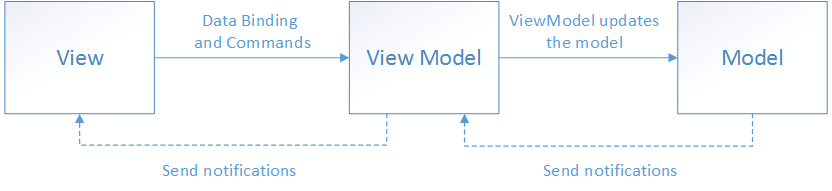
\includegraphics[scale=0.5]{pics/mvvm-pattern.png}
  \caption{Die Model-View-ViewModel Pattern \cite{MVVM}}
  \label{fig:tech:front:mvc-architecture}
\end{figure}

\emph{View} funktioniert hierbei ähnlich wie beim MVC-Pattern, jedoch ist es möglich, dass eine View auch Logik enthält, die Änderungen am Aussehen durchführt. Daher ist das HTML-Template einer Angular-Komponente noch ähnlicher zu dem Konzept einer View aus dem MVVM-Pattern als zu einer View aus dem MVC-Pattern. 

Im ViewModel wird die Funktionalität der Benutzeroberfläche bestimmt. Dabei informiert das ViewModel die View über Änderungen im Model und beliefert es mit Daten. Dieser Vorgang beschreibt das Konzept des Data-Bindings (siehe Data-Binding) in Angular.  

Das Model funktioniert im Grunde gleich wie beim MVC-Pattern, nur wird hierbei nicht die View, sondern das ViewModel über Änderungen informiert. Somit ist das ViewModel das Mittelstück zwischen View und Model.

Angular nutzt hierbei eine Mischung aus beiden Architecture-Patterns. Diese Architektur wird durch das Konzept von Komponenten realisiert, in den nächsten Kapiteln, besonders im Kapitel Umsetzung der Landingpage \ref{landingpage implentation} näher eingegangen. Dabei werden die Parallelen der Patterns erkennbar.
\cite{MVVM}

\paragraph{NgModules [M]}\label{sec:NgModules}
\setauthor{Fabian Maar}
NgModules erleichtern die Einbindung von Libraries. Da keine externen Dateien mühsam heruntergeladen und eingebunden werden müssen und jeder Import-Prozess durch wenige Zeilen Code erfolgt, wird Zeit beim Entwickeln gespart. Alle Importe werden in chronologischer Reihenfolge gelistet, wodurch ein guter Gesamtüberblick geliefert wird und schnell überflüssige Imports entfernt werden können. Die kontinuierliche Erweiterung und die Unterstützung von Third-Party-Libraries, die unter anderem für die 3D-Darstellung verwendet werden, wird ebenfalls von diesen ngModulen ermöglicht. Die Angular-Applikation wird hierbei organisiert und gestartet, in dem die Metadaten wie folgt abgespeichert werden:

\begin{itemize}
  \item Declarations - In dieser Sektion werden alle zugehörigen Komponenten, Direktiven und Pipes deklariert 
  \item Providers - Sie initialisieren wie die Werte bei der Dependency Inection (siehe Dependency Injection \ref{DPI})abgerufen werden \cite{AngularProviders}
  \item Imports - Hier werden alle Libraries und exportierte Modules importiert
  \item Exports - Sie beinhalten alle zu exportierenden Module
  \item Bootstrap - Hierbei wird angegeben welche Komponente beim Anwendungsstart zuerst geladen wird
\end{itemize}

Wie die ngModules verwendet in der 3D-Gallerie-Applikation wurden, wird im Abschnitt Routing (siehe Routing \ref{lst:impl:routing}) nochmals erklärt.
\cite{AngularNgModules}
\cite{AngularNgModulesAPI}
\cite{AngularBuch}


\subsubsection{Angular Schlüsseltechnologien [L]}
Angular ist ein hochanpassbares Framework. Bei der Verarbeitung von asynchronen Prozessen und Events kann Angular um die Library RxJS erweitert werden. Bei der Paketierung und beim Update von geändertem Code wird der Entwickler von der Libary Webpack unterstützt. Das Framework besitzt eine umfassende und äußerst umfangreiche Dokumentation im Web.
\setauthor{Litzlbauer Lorenz}
\paragraph{RxJS [L]}
\begin{wrapfigure}{r}{0.3\textwidth}
  \begin{center}
    
\includegraphics[width=0.2\textwidth]{pics/RxJs_logo.png}
   \caption{RxJS Logo}
  \end{center}
\end{wrapfigure}
RxJS ist eine Implementierung von ReactiveX für die Programmiersprache Javascript.

ReactiveX ist eine Library für das Erstellen von asynchronen und Event-basierten Programmen, dafür benutzt es \emph{observable sequences}. Ein beobachtetes Subjekt führt eine Liste von den Observern. Bei einer Veränderung im Subjekt werden die Beobachter nach der Reihenfolge der Liste über die Veränderung informiert. (Siehe im Glossar \ref{txt:glos:observerDesignPattern} auf Seite \pageref{txt:glos:observerDesignPattern}).
Die Library arbeitet so mit dem \emph{Observer-Design-Pattern} und fügt verschiedene neue Operatoren hinzu. Zusätzlich werden Low-Level-Funktionen wie Threading, Synchronisation und Thread-Sicherheit verarbeitet und keine Input-/Output-Prozesse blockiert. \cite{ReactiveXIntro}

\paragraph{Webpack [L]}
\begin{wrapfigure}{r}{0.3\textwidth}
  \begin{center}
    
\includegraphics[width=0.2\textwidth]{pics/webpack-logo.png}
   \caption{Webpack Logo}
  \end{center}
\end{wrapfigure}
Die Hauptfunktion von Webpack ist es, viele verschiedene Daten zu einem Paket für eine JavaScript Applikation zusammenzufassen.
Angular benutzt Webpack, um TypeScript in JavaScript und Sass bzw. Scss in Css umzuwandeln. Beim Bauen des Projektes werden alle Module in ein einziges zusammengefasst. Bei der Entwicklung der Applikation wird durch Webpack \emph{Live-Reloading} unterstützt. Dabei wird bei einer Änderung im Code die gesamte Applikation aktualisiert und neu gestartet. \cite{Webpack}

\subsection{User-Interface-Frameworks (UI-Frameworks) [L]}
Ein User-Interface-Framework ist eine Ansammlung von Web Komponenten wie z.B. eine Navigationsleiste die sofort im Projekt nutzbar ist.


Die Vorteile von UI-Frameworks sind:\cite{CssFrameworkExplaination, BestCSSFrameworksin2022}
\begin{compactitem}
    \item vereinfacht und beschleunigt den Entwicklungsprozess;
    typische Web-Komponenten sind vordefinierte, der Entwickler muss diese nicht mehr implementieren und erspart sich Zeit.
    \item Cross-Browser Unterstützung;
    Besonders bei neuen CSS-Feature kann es sein, dass diese noch nicht von allen Browsern unterstützt werden. Ein UI-Framework benutzt in der Regel nur Funktionen, die auch alle Browser anzeigen können.
    \item Der Code hat eine bessere Lesbarkeit;
    In einem UI-Framework gibt es gewisse Konventionen wie Klassennamen, die befolgt werden müssen. Dadurch wird der Code besser lesbar.
\end{compactitem}


Die Nachteile von UI-Frameworks sind: \cite{CssFrameworkExplaination, BestCSSFrameworksin2022}
\begin{compactitem}
    \item Die Ladezeit der Webseite erhöht sich;
    Schließlich müssen auch mehr Daten an den Browser geschickt werden.
    \item Webseiten, die das selbe UI-Framework verwenden, schauen einander ähnlich aus;
    Da die Web-Komponenten gleich implementiert werden.
\end{compactitem}


\subsection{UI-Frameworks im Projekt [L]}
Im Projekt wurde sich für zwei UI-Frameworks, Bootstrap und AngularMaterials, entschieden.


\subsubsection{Angular Material [L]}
\begin{wrapfigure}{r}{0.3\textwidth}
  \begin{center}
    
\includegraphics[width=0.2\textwidth]{pics/Angular_Material_UI_Logo.png}
   \caption{Angular Material UI Logo}
  \end{center}
\end{wrapfigure}
Angular Material ist eine UI Framework und wird seit 2014 von Google entwickelt. Das Framework baut auf Angular auf und erweitert es mit eigenen Komponenten, Styleguides, Typographie und vielem mehr. Die Design-Sprache orientiert sich dabei an der \emph{Material Design Spezifikation} von Google. Ein großer Fokus des Frameworks ist die Responsiveness, Komponenten werden auf verschiedenen Auflösungen gut aussehen. \cite{JavaPointAngularMaterial, WhatAngularMaterial}


Angular Material hat folgende Features: \cite{JavaPointAngularMaterial, WhatAngularMaterial}
\begin{compactitem}
    \item Erweiterbar; Bei der Installation lassen sich viele Designanpassungen machen, zusätzlich lassen sich Styles mit dem globalen Stylesheet überschreiben. 
    \item Hochwertig; Die Komponenten sind erprobt und wurden auf die Performanz und Verlässlichkeit getestet.
    \item Reibungslos; Angular Material ist gut mit Angular integriert
\end{compactitem}

Angular Material bietet eine hohe Anzahl an sofort einsetzbaren Komponente. Zu allen diesen Komponenten gibt es auf der offizielle Webseite eine ausführliche Dokumentation mit Beispiele. \cite{JavaPointAngularMaterial, WhatAngularMaterial}

\paragraph{Material Design Spezifikation [L]}
Material Design ist ein Styleguide der von der Firma Google entwickelt wurde. Er soll dabei helfen qualitative hochwertige digitale Produkte für Android, iOS, Flutter und das Web zu gestalten.

Material Design hat mehrere Prinzipien, die sie ihr Design beeinflussen lassen.

Material Design soll die reale Weld abbilden.
Text soll durch Typographie, Raster, Abstände, Farben und Bilder soll eine erkennbare Hierarchie entstehen. Komponenten sind interaktive Bauklötze für ein das User Interface. Komponenten haben alle eine Stati-System welches den Status der Komponente fokussiert, selektiert, aktiviert, fehlerhaft, schwebend, gedrückt und ausgeschalten anzeigt. Durch das Theming ist es möglich einzelne Komponenten zu verändern und das Design so anzupassen, dass es zur Corporate Identity der Benutzer*in passt.\cite{MaterialDesign-Introduction}

\paragraph{Angular Material Komponente im Projekt [L]}

\begin{figure}
  \centering
  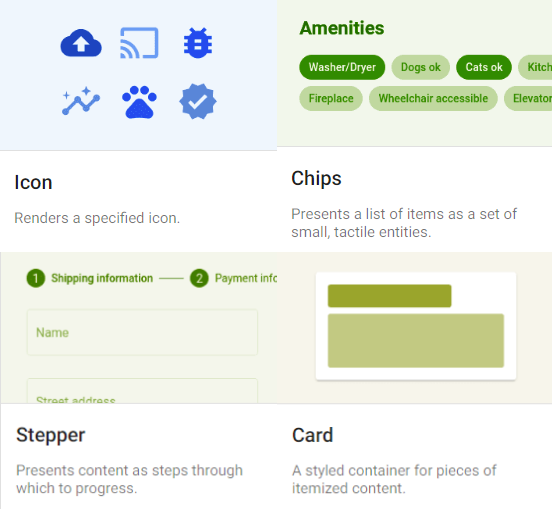
\includegraphics[scale=0.5]{pics/AngularMaterialKomponent.png}
  \caption{Angular Material: Komponenten die im Projekt verwendet wurden \cite{AngularComponents}}
  \label{architecture:frontend:angular-material-project-components}
\end{figure}

Im Projekt wurden hauptsächlich die Angular Material Komponenten mat-icon, mat-chips, mat-stepper und mat-chard verwendet (siehe Abbildung \ref{architecture:frontend:angular-material-project-components}).

mat-icon wird dafür verwendet, die Icons auf der SPA anzuzeigen. Die Icons werden durch den Inhalt, den Namen des Icons im mat-icon ausgewählt.

mat-chips werden für das Design der Ausstellungskriterien benützt. Sie kommen in der Content-Creation und der Suchseite hauptsächlich vor.

mat-stepper wird bei der Content-Creation verwendet, um die Wizard-Funktion umzusetzen.

mat-chard wird für die Ausstellungsstückkarten auf der SPA verwendet. Diese kommen auf der Profile-, Such- und Landing-Page vor.

\subsubsection{Bootstrap [L]}
\begin{wrapfigure}{r}{0.3\textwidth}
  \begin{center}
    
\includegraphics[width=0.2\textwidth]{pics/Bootstrap_logo.png}
   \caption{Bootstrap Logo}
  \end{center}
\end{wrapfigure}
Bootstrap ist ein kostenloses Open-Source-UI-Framework. Es ist nicht nur eine Ansammlung von CSS sondern auch von JavaScript und HTML code um schöne, interaktive und responsive Webseiten.  \cite{BestCSSFrameworksin2022}

Bootstrap hat folgenden Features:  \cite{BestCSSFrameworksin2022}
\begin{compactitem}
    \item Web-Komponenten, die sofort Anwendbar sind
    \item Eine gute Dokumentation
    \item Mobile Centered Design
    \item Hohe Benutzerfreundlichkeit
\end{compactitem}

\subsubsection{SCSS [L]}
\begin{wrapfigure}{r}{0.3\textwidth}
  \begin{center}
    
\includegraphics[width=0.2\textwidth]{pics/Sass_Logo.png}
   \caption{Sass Logo}
  \end{center}
\end{wrapfigure}
SCSS ist kein UI-Framework, sondern vielmehr eine Syntax- und Feature-Erweiterung von CSS, deswegen wurde es schlussendlich auch für dieses Projekt gewählt. SCSS hat viele Vorteile wie zum Beispiel Variablen, Schleifen, Mixins und Imports gegenüber CSS, aber besonders ausschlaggebend war das Prinzip der Verschachtelung. \cite[Sass Guide]{SassGuide}

Durch die Verschachtelung kann an redundanten Styles-Selektoren gespart werden, was die Style-Definition besser lesbarer macht. Im den Beispielen (siehe SCSS-Code-Beispiel \ref{lst:imp:design:scss} und natives CSS-Code-Beispiel \ref{lst:imp:design:css}) wird die gleiche Style-Definition von SCSS und CSS ausgedrückt, doch die Schreibweise unterscheidet sich. \cite[Sass Guide]{SassGuide}

\cite[Sass Guide]{SassGuide}


\begin{lstlisting}[caption=SCSS - Code Beispiel,label=lst:imp:design:scss]
nav {
    ul {
        margin: 0;
        padding: 0;
        list-style: none;
    }
    
    li { display: inline-block; }
    
    a {
        display: block;
        padding: 6px 12px;
        text-decoration: none;
    }
}
\end{lstlisting}

\begin{lstlisting}[caption=CSS - Code Beispiel,label=lst:imp:design:css]
nav ul {
    margin: 0;
    padding: 0;
    list-style: none;
    }
nav li {
    display: inline-block;
    }
nav a {
    display: block;
    padding: 6px 12px;
    text-decoration: none;
}
\end{lstlisting}

Code Beispiele\ref{lst:imp:design:scss} \ref{lst:imp:design:css} \cite[Sass Guide]{SassGuide}

\subsection{3D Rendering [L]}
Es gab verschiedene Auswahlkriterien für die 3D-Web-API, die ausschlaggebend für den Projekterfolg waren:
\begin{compactitem}
  \item Effizienzen der 3D Engine (Hardware Acceleration, RAM-Auslastung)
  \item Benutzerfreundlichkeit (Programmerexperience)
  \item Das Laden von 3D-Modellen aus 3D-Dateien und aus dem Internet
  \item Video-Texturen support
\end{compactitem}

\subsubsection{ThreeJs [L]}
\setauthor{Litzlbauer Lorenz}
\begin{wrapfigure}{r}{0.3\textwidth}
    \begin{center}
      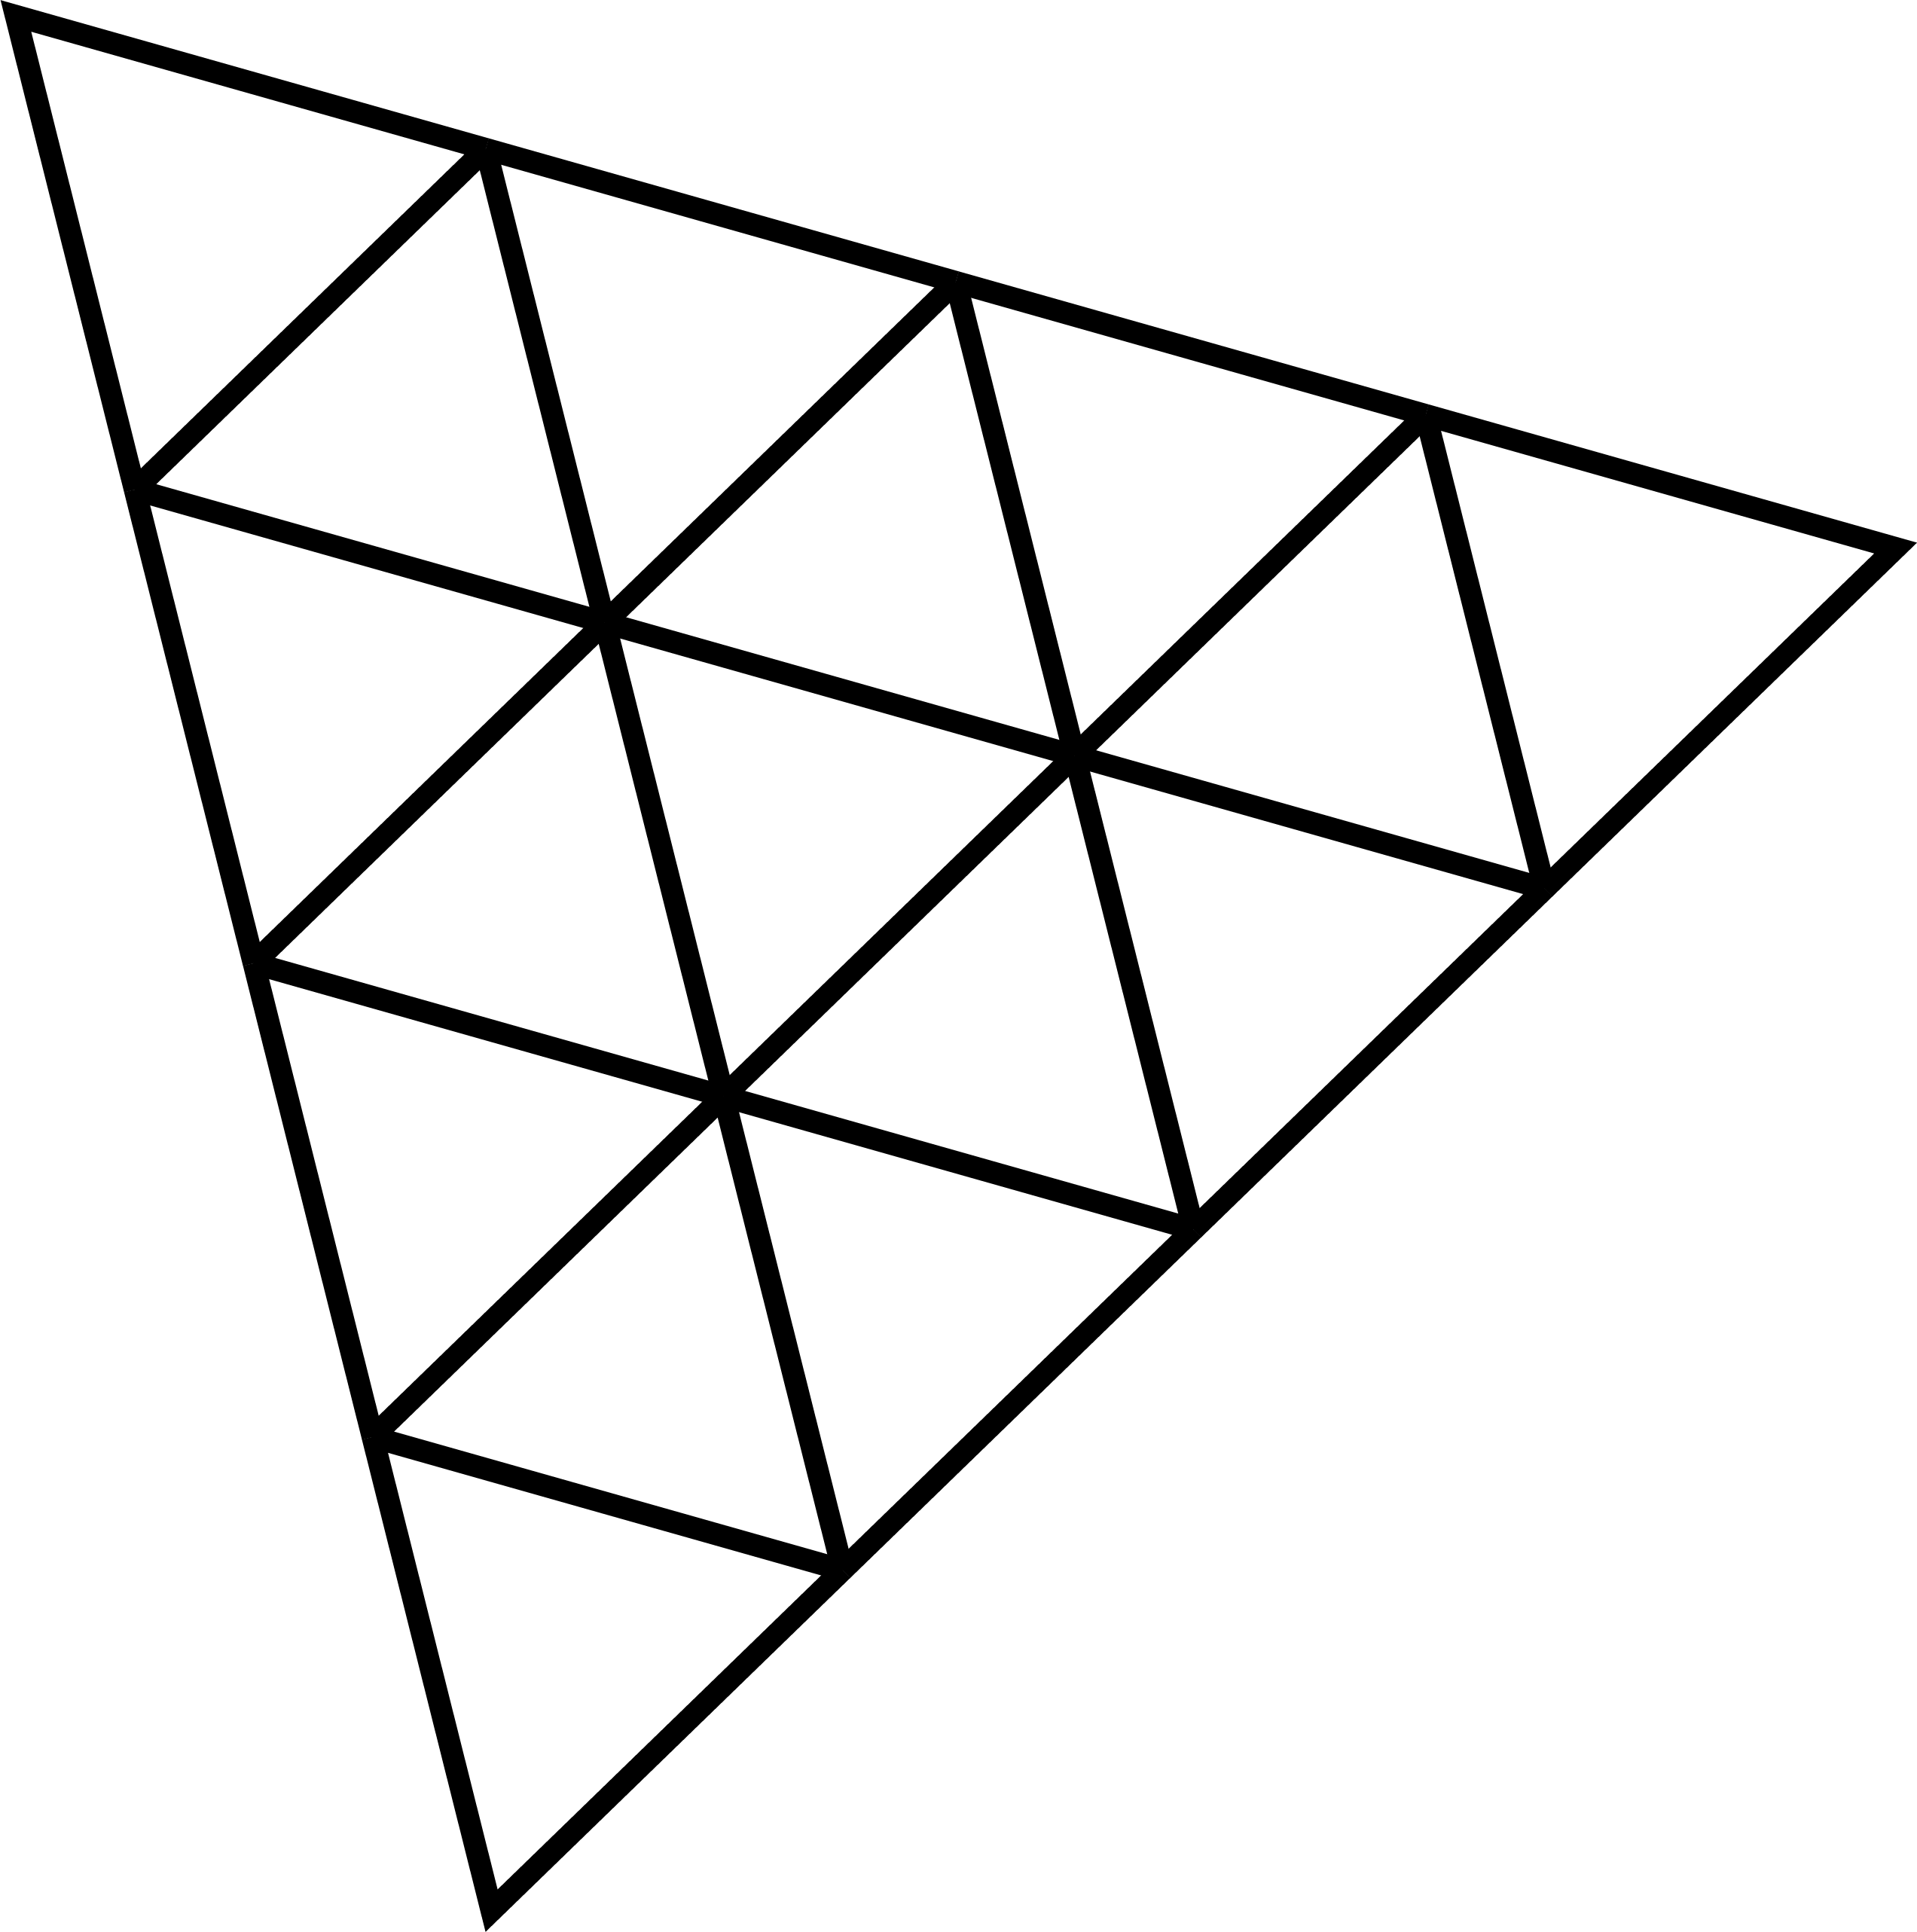
\includegraphics[width=0.2\textwidth]{pics/threeJS.png}
     \caption{ThreeJs Logo}
    \end{center}
\end{wrapfigure}
ThreeJs ist eine JavaScript Library für die Darstellung von 3D-Grafiken im Web. Für die 3D-Darstellung nutzt ThreeJs WebGL (mehr dazu im nächsten Abschnitt \hyperref[ch::webgl]{WebGL}), ein Low-Level-Framework. WebGL hat eine hohe Komplexität. ThreeJs bietet eine Abstraktion von WebGL, um Anwendungen für 3D-Webanwendungen für Entwickler zugänglicher zu machen.
ThreeJs regelt Systeme wie die 3D-Szene, Lichter, Schatten, Materialien, Texturen und 3D-Matrix-Rechnungen, deren Umsetzung mittels WebGL sehr aufwändig wäre. \cite[ThreeJs fundamentals]{ThreeJsFund}

\begin{figure} [h t]
  \centering
  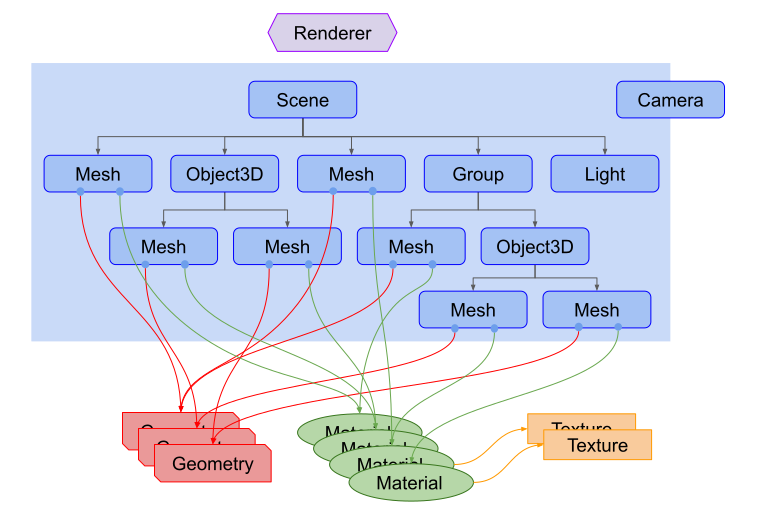
\includegraphics[scale=0.5]{pics/threejs-structure.png}
  \caption{Die Struktur von ThreeJs \cite{ThreeJsFund}}
  \label{fig:tech:front:threejsstructure}
\end{figure}

In ThreeJs werden Geometrie, Objekte und Materialien verbunden, um ein 3D-Objekt zu erstellen. 
Die Abbildung \ref{fig:tech:front:threejsstructure} veranschaulicht den beispielhaften Aufbau eines solchen Objektes. In diesem Objekt werden Meshes, Gruppen, Lichter und 3D-Objekte in einer Baumdatenstruktur gesammelt. Die Daten über die Geometrie, Materialen der Meshes werden außerhalb der Szene gespeichert und die Meshes referenzieren im Renderprozess darauf. \cite[ThreeJs fundamentals]{ThreeJsFund}

\label{ch::ThreeJsDependency}
Um 3D-Darstellungen zu rendern, benutzt ThreeJs WebGL.

\paragraph{WebGL [L]}
\label{ch::webgl}
\begin{wrapfigure}{h  r}{0.3\textwidth}
    \begin{center}
      
\includegraphics[width=0.2\textwidth]{pics/WebGL_Logo.png}
     \caption{WebGL Logo}
    \end{center}
\end{wrapfigure}
WebGL ist eine lizenzfreie Low-Level-API, die dafür benutzt wird, 3D-Grafiken im Web darzustellen. Sie basiert auf OpenGL ES 2.0 und benutzt auch dieselbe Grafik-Programmiersprache, wie Open GLSL (OpenGL Shading Language). Eine Low-Level-API hat einen höheren Konfigurierungsgrad und lässt sich für spezielle Anwendungsfälle besser anpassen. Die API setzt ein viel tieferes Verständnis von dem Material (WebGL Shader-Programmierung, Matrixrechnungen usw.) voraus und bringt somit einen höheren Programmieraufwand mit sich. \cite{WebglGettingStarted, HighlowAPI}

\subsubsection{Alternative 3D Web APIs [L]}
Es gibt viele Technologien, die 3D-Grafiken im Web ermöglichen, wie Three.js, Babylon.js, A-Frame, X3DOM und WebGL.

\paragraph{A-Frame [L]}
A-Frame wird von der Mozilla Foundation als OpenSource-Projekt entwickelt. Die 3D-Szene wird durch eine deklarative Sprache mit XML-Syntax definiert. Über die WebVR-API bietet die Libray auch die Möglichkeit, 3D-Szenen durch eine VR-Brille zu erfahren. Bei der 3D-Darstellung setzt A-Frame auf ThreeJs. \cite[A-Frame Wikipedia]{a-frame-wiki}

A-Frame hat ähnliche Funktionen und Leistung im Vergleich zu ThreeJs, da es ja schlussendlich darauf aufbaut. A-Frame sticht bei der VR support hervor (ThreeJs hätte auch eine Unterstützung dafür, diese ist aber schwieriger einzubinden), doch ist das kein unbedingt nötiges Feature. ThreeJs ist ja bereits eine Abstraktion von WebGL. Für das Projekt wird keine weiter Abstraktion gebraucht.

\subsubsection{Angular Three [L]}
\label{ch:Technologien:AngularThree}
Angular Three ist ein Open Source Projekt von Matt DesLauriers. Es zielt darauf ab die Vorteile von Angular und ThreeJs zu kombinieren. Dabei verbindet es das Prinzip der Komponenten von Angular mit der 3D Darstellung von ThreeJs. 

\begin{lstlisting}[language=html,caption=Angular Three - Komponentenbasiertes 3D Scenen in HTML,label=lst:impl:AngularThreeExampleCode]
<ngt-canvas>
    <ngt-ambient-light intensity="0.5"></ngt-ambient-light>
    <ngt-spot-light [position]="10" angle="0.15" penumbra="1"></ngt-spot-light>
    <ngt-point-light [position]="-10"></ngt-point-light>
  
    <app-cube [position]="[1.2, 0, 0]"></app-cube>
    <app-cube [position]="[-1.2, 0, 0]"></app-cube>
  
    <ngt-soba-orbit-controls></ngt-soba-orbit-controls>
</ngt-canvas>
\end{lstlisting}

\begin{lstlisting}[language=html,caption=Angular Three - App Cube,label=lst:impl:AngularThreeCube]
<ngt-mesh
  (beforeRender)="onCubeBeforeRender($event)"
  (click)="active = !active"
  (pointerover)="hovered = true"
  (pointerout)="hovered = false"
  [scale]="active ? 1.5 : 1"
  [position]="position"
>
  <ngt-box-geometry></ngt-box-geometry>
  <ngt-mesh-standard-material [color]="hovered ? 'turquoise' : 'tomato'"></ngt-mesh-standard-material>
</ngt-mesh>
\end{lstlisting}

Code Beispiele \ref{lst:impl:AngularThreeExampleCode} \ref{lst:impl:AngularThreeCube} \cite{AngularThreeDocumentationFirstScene}

Ein Vorteil von Angular Three ist, dass durch nur wenige Zeilen Code \ref{lst:impl:AngularThreeExampleCode} eine 3D-Szene mit Lichtern und Orientierungsfunktionen erstellt werden kann und die Business-Logik, App-Cube \ref{lst:impl:AngularThreeCube} durch die Verwendung einer Komponente ausgelagert werden kann.

Ein weiterer Vorteil von Angular Three ist die ausführliche Dokumentation mit Codebeispielen. \href{https://angular-three.netlify.app/docs/getting-started/overview}{(link) Angular Three Dokumentation https://angular-three.netlify.app/docs/getting-started/overview}

Wegen der vielen Vorteile hohe Benutzerfreundlichkeit, ähnliche 3D-Leistung zu ThreeJs (Angular Three basiert auf ThreeJs, welches selbst die WebGL-Renderengine benutzt) und wegen der Verbindung von Angular und ThreeJs Features bietet sich die Liberay für das Projekt an.

Mithilfe eines Prototypen ( mehr dazu im Abschnitt \hyperref[ch::ongoing-prototyping]{fortlaufendes Prototyping} ) wurde getestet, ob Angular Three alle Features, die für das Projekt benötigt werden, unterstützen kann, die für das Projekt nötig sind. Dabei wurde festgestellt, dass sich die Library Angular Three für das Projekt nicht eignet. Trotz der vielen Features konnten einige Kriterien nicht erfüllt werden. So wurden beispielsweise 3D-Objekte nicht richtig geladen. ThreeJs Module funktionierten Teilweise nicht, wie die FristPersonControls. 

Weil Angular Three nicht die für das Projekt aufgestellten Anforderungen erfüllt hat, wurde sich dafür entschieden, ThreeJs zu benutzen. ThreeJs hat ähnliche Konzepte und Logik wie Angular Three deswegen fiel dem Team der Umstieg darauf leicht. Diese 3D-Library wurde schlussendlich auch im Projekt verwendet.

\subsection{Sicherheit [L]}
\setauthor{Litzlbauer Lorenz}

\subsection{JWT - Json Web Token [L]}
\begin{wrapfigure}{r}{0.3\textwidth}
  \begin{center}
    
\includegraphics[width=0.2\textwidth]{pics/jwt_logo.png}
   \caption{JWT Logo}
  \end{center}
\end{wrapfigure}
Der Json Web Token (JWT) ist ein offenerer Standard. Er wird durch RFC 7519 definiert. JWT wird zur sicheren Übertragung von Informationen über ein JSON-Objekt benutzt, indem er den*die Benutzer*in authentifiziert. Die Authentifizierung passiert meist am Server. Dort wird nach einer Validierung der Token digital unterschrieben, entweder durch ein Passwort und eine Hashfunktion wie HMAC oder durch ein asymmetrisches Kryptosystem wie RSA. \cite{jwtAuth0}


